\section{Creare un proprio stile per la Tesi}
In questa sezione analizzeremo come creare un proprio stile per una Tesi di
laurea. È risaputo infatti come una pubblicazione di questo calibro possa
essere corposa. Come accennato all'inizio della guida, \LaTeX{} è
particolarmente adatto per documenti di certe dimensioni, e qui vedremo come
creare uno stile per la tesi di laurea.

\subsection{Copertina}
Anche se di importante in una tesi è il contenuto, anche l'occhio vuole la sua
parte. La realizzazione di una copertina non è difficile, e qui vedremo come
realizzarla in pochi passi, strutturando il progetto come abbiamo visto nel
capitolo apposito. % TODO mettere un ref per il capitolo 2

Prima di tutto, definiremo dei comandi in maniera tale da rendere la creazione
della copertina più chiara e anche per separare il contenuto dalla
presentazione.

\paragraph*{Creazione delle variabili} Apriamo il nostro file
\texttt{res/config/config.tex} e aggiungiamo le nostre generalità sottoforma di
variabili:

\lstinputlisting{res/examples/tesi/config.tex}

\paragraph*{Creazione del frontespizio} Ora che abbiamo creato le variabili con
le nostre informazioni andiamo a creare la parte grafica, ovvero quella che poi
sarà generata come prima pagina. Per far ciò creiamo un file in
\texttt{res/sections/Frontespizio.tex} e aggiungiamo il seguente contenuto:

\lstinputlisting{res/examples/tesi/frontespizio.tex}

\noindent Ora abbiamo la copertina per la nostra tesi.

\begin{figure}[t]
 \centering
 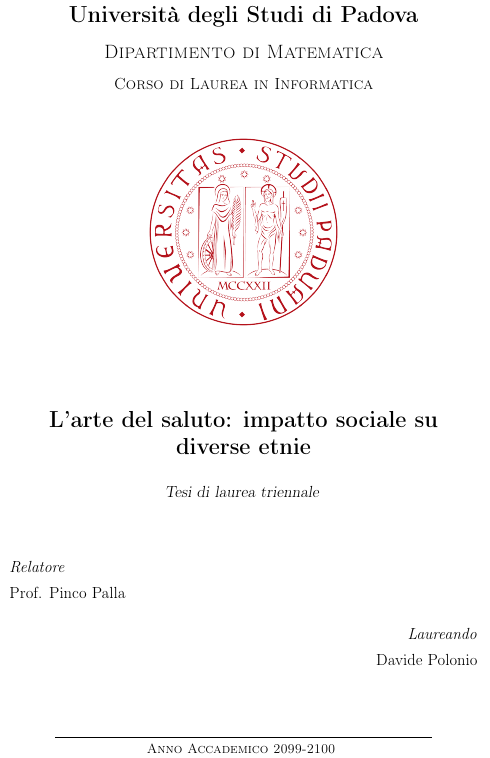
\includegraphics[scale=0.5]{thesis_frontispiece}
 \caption[Frontespizio tesi]{Risultato della copertina che abbiamo appena
scritto}
 \label{img:thesis_frontispiece}
\end{figure}


\subsection{Seconda pagina, ringraziamenti}
Come tutte le tesi che si rispettino, è importante anche introdurre prima
quello che viene definito come \textbf{colofone} (ovvero una parte in cui sono
scritti i dettagli della pubblicazione) e poi una sezione di ringraziamenti.
Andremo ora a vedere come si fa.
\paragraph*{Colofone} Prima di tutto, andiamo a creare un altro
file, nel percorso \texttt{res/sections} e chiamiamolo \texttt{colofone}.
Ricordiamoci di includere questo file aggiungendolo al file
\texttt{listOfSections.tex} che, se abbiamo seguito la guida passo passo, si
trova in \texttt{res/}.

\lstinputlisting{res/examples/tesi/colofone.tex}

\paragraph*{Ringraziamenti} Creiamo un altro file nel solto percorso, e lo
chiameremo \texttt{ringraziamenti.tex}. Qui inseriremo la dedica che più ci
piace, completata dalla nostra firma che sarà in basso a destra.

\lstinputlisting{res/examples/tesi/ringraziamenti.tex}

\subsection{Riferimenti bibliografici}

Abbiamo già visto in altre parti del testo come eseguire riferimenti
bibliografici. Ora andremo a crearlo usando \textbf{Bibtex}.

Creiamo un file in \texttt{res/bibliography.bib}, e aggiungiamo le nostre fonti
con la seguente sintassi:

\lstinputlisting{res/examples/tesi/bibliografia.bib}

\noindent A questo punto dovremo specificare nelle impostazioni che abbiamo
aggiunto queste voci. Apriamo di nuovo il nostro file di configurazione (che
ricordiamo si trova in \texttt{res/config/config.tex}) e aggiungiamo il
seguente codice:

\lstinputlisting{res/examples/tesi/config2.tex}

\noindent Bene! Ora abbiamo aggiunto i riferimenti bibliografici alla nostra
tesi.

\section{Si può fare di più?}

Certo! Si possono certamente aggiungere delle appendici a fine tesi (con il
comando \verb!\appendix! si segnala l'inizio della sezione dedicata alle
appendici) e anche l'aggiunta di un glossario dei termini potrebbe aiutare il
lettore a comprendere di più quello che è stato scritto.
Queste parti possono essere approfondite rispettivamente in:
\begin{itemize}
 \item
\url{https://en.wikibooks.org/wiki/LaTeX/Document_Structure#Book_structure}
 \item \url{https://en.wikibooks.org/wiki/LaTeX/Glossary}
\end{itemize}

